% =====================================================================
%  論文1（日本語稿）正典ソース
%  基点分岐：扁長回転楕円体上で停留円が中心へ収縮する臨界軸比
%
%  組版: LuaLaTeX + luatexja (ltjsarticle)
%  コンパイル: latexmk -lualatex Paper1_Japanese.tex
%             （または lualatex を2回）
%
%  図: figures/fig1_local_bifurcation.pdf
%      figures/fig2_shrinking_circle.png
%      matplotlib の PDF 出力をそのまま置く。PNG しかない場合は
%      拡張子を .png に変更してよいが、PDF を推奨。
% =====================================================================
\documentclass[a4paper,11pt]{ltjsarticle}

\usepackage{amsmath}
\usepackage{amssymb}
\usepackage{amsthm}
\usepackage{graphicx}
\usepackage[margin=25mm]{geometry}
\usepackage[unicode,hidelinks]{hyperref}

\theoremstyle{plain}
\newtheorem{thm}{定理}[section]
\newtheorem{prop}{命題}[section]
\theoremstyle{definition}
\newtheorem{dfn}{定義}[section]

\newcommand{\leadin}[1]{\medskip\noindent\textbf{#1}\quad\ignorespaces}

\title{基点分岐：扁長回転楕円体上で\\
停留円が中心へ収縮する臨界軸比\\[2mm]
\large — 錐体積重み付き動径–法線角に対する区間認証 —}
\author{古田 勝士 / Katsushi Furuta\\ Independent Researcher}
\date{2026年8月23日}

\begin{document}
\maketitle

\leadin{論文の核心。}
本稿は、対象の変形に伴って停留集合が組み変わる「基点分岐」の実在を証明する。

\leadin{草稿の状態。}
主定理は、局所係数 \(Q, H_4\) と臨界軸比 \(a_c\) の区間認証、および局所分岐解析だけで
閉じている。全域完全性の検証は主定理の投稿条件ではなく、大域完全性を扱う続編の課題とする。

\begin{abstract}
凸体に付随する錐体積重み付き動径–法線角汎関数について、基点を可動変数として扱い、その停留集合が
扁長回転楕円体の軸比に応じて組み変わることを示す。回転対称性により中心は常に停留点であるが、ある
臨界軸比の一側には赤道面内の停留円が現れ、臨界値へ近づくにつれて中心へ収縮する。局所還元により、
二次係数 \(Q(a)\) の単純零点 \(a_c\) と四次係数 \(H_4(a_c)<0\) を区間演算で認証し、停留円の存在・
一意性・収縮則を導く。

本稿の主張は、珍しい停留集合の報告そのものではない。パラメータ付き停留集合の局所的な射影が、成分
次元・法方向モース指数・nullity・等方型を保存する局所自明化を失うことを「基点分岐」と定義し、この
現象が実在することを証明する点にある。必要な計算機援用部分は、局所係数の区間評価、固定された入力と
実行環境、および fail-closed な符号判定によって証明へ組み込む。本稿は存在を扱い、全パラメータ域に
おける完全列挙は別稿に譲る。
\end{abstract}

\noindent\textbf{キーワード：}基点分岐、停留円、Morse–Bott、扁長回転楕円体、区間演算、計算機援用証明

\section{序論}
本稿では、基点を幾何学的変数として扱う。対象に付随する汎関数を固定したうえで基点を動かし、そこに
現れる停留点構造を取り出す。そして対象を変形させたとき、その構造がどう組み変わるかを調べる。

凸体の中心を選ぶ理論は、重心、曲率中心、各種の radial center など、基点を一つの代表点として抽出する
方向に発展してきた。とりわけ一意性を仮定すれば、対称性は中心を対称軸上の点へ拘束する。この成功は
同時に、一意性が破れたときに現れる正の次元の停留集合を視界の外へ置く。連続対称性のもとでは、軸から
離れた一つの停留点は群軌道をなし、孤立点ではなく円として現れうる。

ここで研究対象とするのは、扁長回転楕円体に対する錐体積重み付き動径–法線角である。軸比を変化させると、
赤道面内に一つの停留円が発生し、臨界軸比で中心へ吸収される。本論文はこの円を認証するだけでなく、
停留集合のラベル構造が変わることを示し、基点分岐の具体例として位置づける。停留点の位置が連続的に
動くだけでは分岐とは呼ばない。変化を測るのは、成分の次元、法方向指数、nullity、等方型である。

本研究は、計算を結果の検証だけでなく、パターンの発見、予想の形成、厳密解析の方向づけにも用いる実験
数学の伝統に位置づけられる \cite{BorweinBailey}。

\leadin{三本の柱。}
主定理＝基点分岐の存在。停留円＝主定理を担う幾何学的素材。局所係数の区間認証＝主張を証明へ変える
手段。この順序を本文全体で維持する。

\section{基点分岐の最小定義}
基点空間を \(P\)、対象の変形パラメータ空間を \(\Lambda\) とし、各 \(\lambda\in\Lambda\) に対して
基点汎関数 \(E_\lambda:P\to\mathbb{R}\) が与えられているとする。本稿が必要とする一般枠組みは、
三つ組 \((P,\Lambda,E)\) のみである。
\begin{gather}
\operatorname{Crit}(E_\lambda)=\{\,p\in P: d_pE_\lambda=0\,\},\\
\mathcal{S}=\{\,(\lambda,p)\in\Lambda\times P: d_pE_\lambda=0\,\},\qquad
\pi:\mathcal{S}\to\Lambda,\qquad \pi(\lambda,p)=\lambda.
\end{gather}

\(\mathcal{S}\) の各連結成分には、(i) 成分次元、(ii) 法方向モース指数、(iii) nullity、(iv) 等方型
からなるラベルを付す。正の次元成分について通常の Morse 指数ではなく法方向指数を用いるのは、停留円が
孤立臨界点ではなく Morse–Bott 型臨界多様体だからである。接方向の零固有値は対称性に由来する。

\begin{dfn}[局所基点分岐]
\((\lambda_0,p_0)\in\mathcal{S}\) とする。\(\lambda_0\) を内点に含む両側近傍 \(I\subset\Lambda\) と
\(p_0\) の近傍 \(U\subset P\) をどのように小さく選んでも、制限射影
\[
\pi:\mathcal{S}\cap(I\times U)\to I
\]
が上記ラベルを保存する局所自明化を持たないとき、\((\lambda_0,p_0)\) を基点分岐点、\(\lambda_0\) を
その基点分岐値と呼ぶ。停留成分の位置の連続移動それ自体は、この定義に含めない。
\end{dfn}

この定義は停留集合の芽に関するものである。したがって、中心から離れた別成分の存在や移動とは独立に、
\((\lambda_0,p_0)\) の任意に小さい近傍で生じるラベル構造の変化を判定できる。本稿が実証するのは、
具体的な汎関数におけるこの局所自明性の破れである。

\section{錐体積重み付き動径–法線角}
滑らかで原点を内部に含む凸体 \(K\subset\mathbb{R}^3\) と基点 \(p\in\operatorname{int}K\) を考える。
境界点 \(x\in\partial K\) における外向き単位法線を \(\nu_K(x)\) とし、
\[
\alpha_{K,p}(x)=\arccos\!\left(\frac{x-p}{\lvert x-p\rvert}\cdot\nu_K(x)\right)
\]
を、基点 \(p\) から境界点 \(x\) への動径方向と外向き法線方向のなす角とする。基点 \(p\) に基づく
正規化錐体積測度を
\[
d\mu_{K,p}(x)=\frac{(x-p)\cdot\nu_K(x)}{3\operatorname{Vol}(K)}\,dA(x)
\]
と定める。発散定理により
\[
\int_{\partial K}(x-p)\cdot\nu_K(x)\,dA(x)=3\operatorname{Vol}(K)
\]
であるから、\(\mu_{K,p}\) は確率測度である。本稿で扱う錐体積重み付き動径–法線角汎関数は
\[
E_K(p)=\int_{\partial K}\alpha_{K,p}(x)^2\,d\mu_{K,p}(x)
\]
である。

\begin{prop}[相似不変性]
\label{prop:similarity}
\(T(x)=sUx+q\)（\(s>0\), \(U\in O(3)\), \(q\in\mathbb{R}^3\)）とする。このとき任意の
\(p\in\operatorname{int}K\) について
\[
E_{T(K)}(T(p))=E_K(p)
\]
が成り立つ。
\end{prop}

角度 \(\alpha\) は相似変換および直交変換で不変である。また錐体積測度の分子では支持距離が \(s\) 倍、
面積要素が \(s^2\) 倍となる一方、分母の体積は \(s^3\) 倍となるため、倍率は厳密に相殺される。よって
正規化錐体積測度も保存される。なお基点座標に関する Hessian は一様スケール \(s\) のもとで
\(s^{-2}\) 倍されるが、\(s^{-2}>0\) であるため、符号、Morse index、nullity は保存される。

\section{扁長回転楕円体と局所還元}
\[
K_a=\left\{(x,y,z)\in\mathbb{R}^3:\ x^2+y^2+\frac{z^2}{a^2}\le 1\right\},\qquad a\ge 1 .
\]
ここで回転軸は \(z\) 軸、赤道面は \(z=0\) とする。\(K_a\) の完全な等長群は \(D_{\infty h}\) である。
\(z\) 軸まわりの \(O(2)\) 作用に加え、赤道面に関する鏡映
\[
\sigma_h:(x,y,z)\mapsto(x,y,-z)
\]
を含む。中心 \(p=0\) は全群で固定されるため、すべての \(a\) で停留点である。赤道面 \(z=0\) 上では
\(\sigma_h\) 不変性から \(\partial_zE_a=0\) が強制され、残る停留条件は半径
\[
r=\sqrt{x^2+y^2}
\]
に関する一変数方程式へ還元される。原点近傍で
\[
E_a(r)=E_a(0)+\frac{Q(a)}{2}r^2+\frac{H_4(a)}{24}r^4+O(r^6)
\]
と展開する。赤道面内の非零停留半径は \(\partial_rE_a(r)=0\) の解であり、鏡映対称性が
\(\partial_zE_a=0\) を与えるため、これは三次元の停留点である。\(Q\) の符号変化と \(H_4\) の符号が
局所分岐を支配し、軸方向 \(O(2)\) 対称性により、\(r>0\) の解一つは円 \(S^1\) 全体の停留点を与える。

\section{臨界軸比の区間認証}
\begin{prop}[認証済み局所係数]
\label{prop:certified}
区間 \((4.72438,\,4.72439)\) 内に \(Q(a_c)=0\) を満たす唯一の \(a_c\) が存在し、
\[
a_c\approx 4.7243834045211334067
\]
である。さらに
\[
Q'(a_c)<0,\qquad H_4(a_c)<0
\]
が成り立つ。
\end{prop}

証明は閉区間上の有理・区間演算により行う。\(Q\) の符号反転と単調性から零点の存在と一意性を得て、
同一区間上で \(Q'\) と \(H_4\) の符号を外向き丸めにより固定する。数値近似値は説明のために掲げるが、
論理的入力は包含区間と符号証明である。

\(E_a(r)\) は \((a_c,0)\) の近傍で \(a\) と \(r\) の実解析関数であり、\(r\) に関して偶関数である。
したがって
\[
\partial_rE_a(r)=r\,G(a,r^2),\qquad
G(a,s)=Q(a)+\frac{H_4(a)}{6}s+O(s^2)
\]
と因数分解できる。ここで剰余は \((a_c,0)\) の十分小さい閉近傍上で一様に制御される。
\(H_4(a_c)\neq 0\) なので、解析的陰関数定理 \cite{GSS} により \(G(a,s(a))=0\)、\(s(a_c)=0\) を満たす
一意な局所枝が存在する。さらに
\[
s'(a_c)=-\frac{6Q'(a_c)}{H_4(a_c)}<0
\]
であるから、\(a<a_c\) 側では \(s(a)>0\)、\(a>a_c\) 側では \(s(a)<0\) となる。ゆえに前者に限って
\(r(a)=\sqrt{s(a)}>0\) が存在し、
\[
r(a)\to 0\qquad (a\uparrow a_c)
\]
である。また
\[
r(a)^2=s(a)=-\frac{6Q(a)}{H_4(a_c)}+O\!\left((a-a_c)^2\right)
\]
であり、停留円の収縮則と反対側での局所非存在が厳密に従う。

\begin{figure}[htbp]
\centering
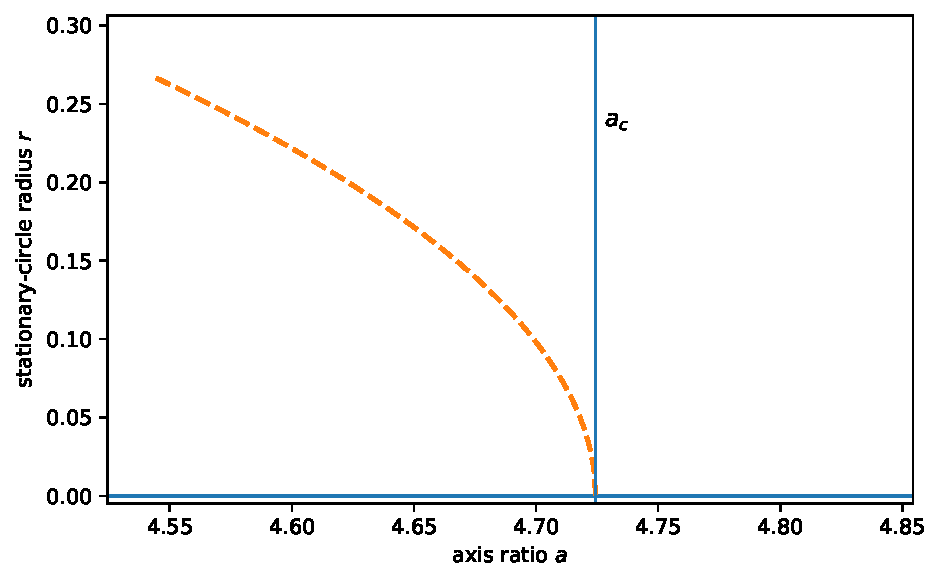
\includegraphics[width=0.85\linewidth]{figures/fig1_local_bifurcation.pdf}
\caption{局所分岐図。中心枝 \(r=0\) は全軸比で存在する。\(Q(a)\approx Q'(a_c)(a-a_c)\) より、破線は
認証済み参照係数 \(c=6Q'(a_c)/H_4(a_c)\approx 0.39474123\) を用いた主項 \(r_*(a)^2=c(a_c-a)\) であり、
実測枝または大域的数値追跡ではない。帯は \(a_c\in(4.72438,4.72439)\) の認証区間を示す。}
\label{fig:bifurcation}
\end{figure}

\section{局所停留円とラベル構造}
\begin{figure}[htbp]
\centering
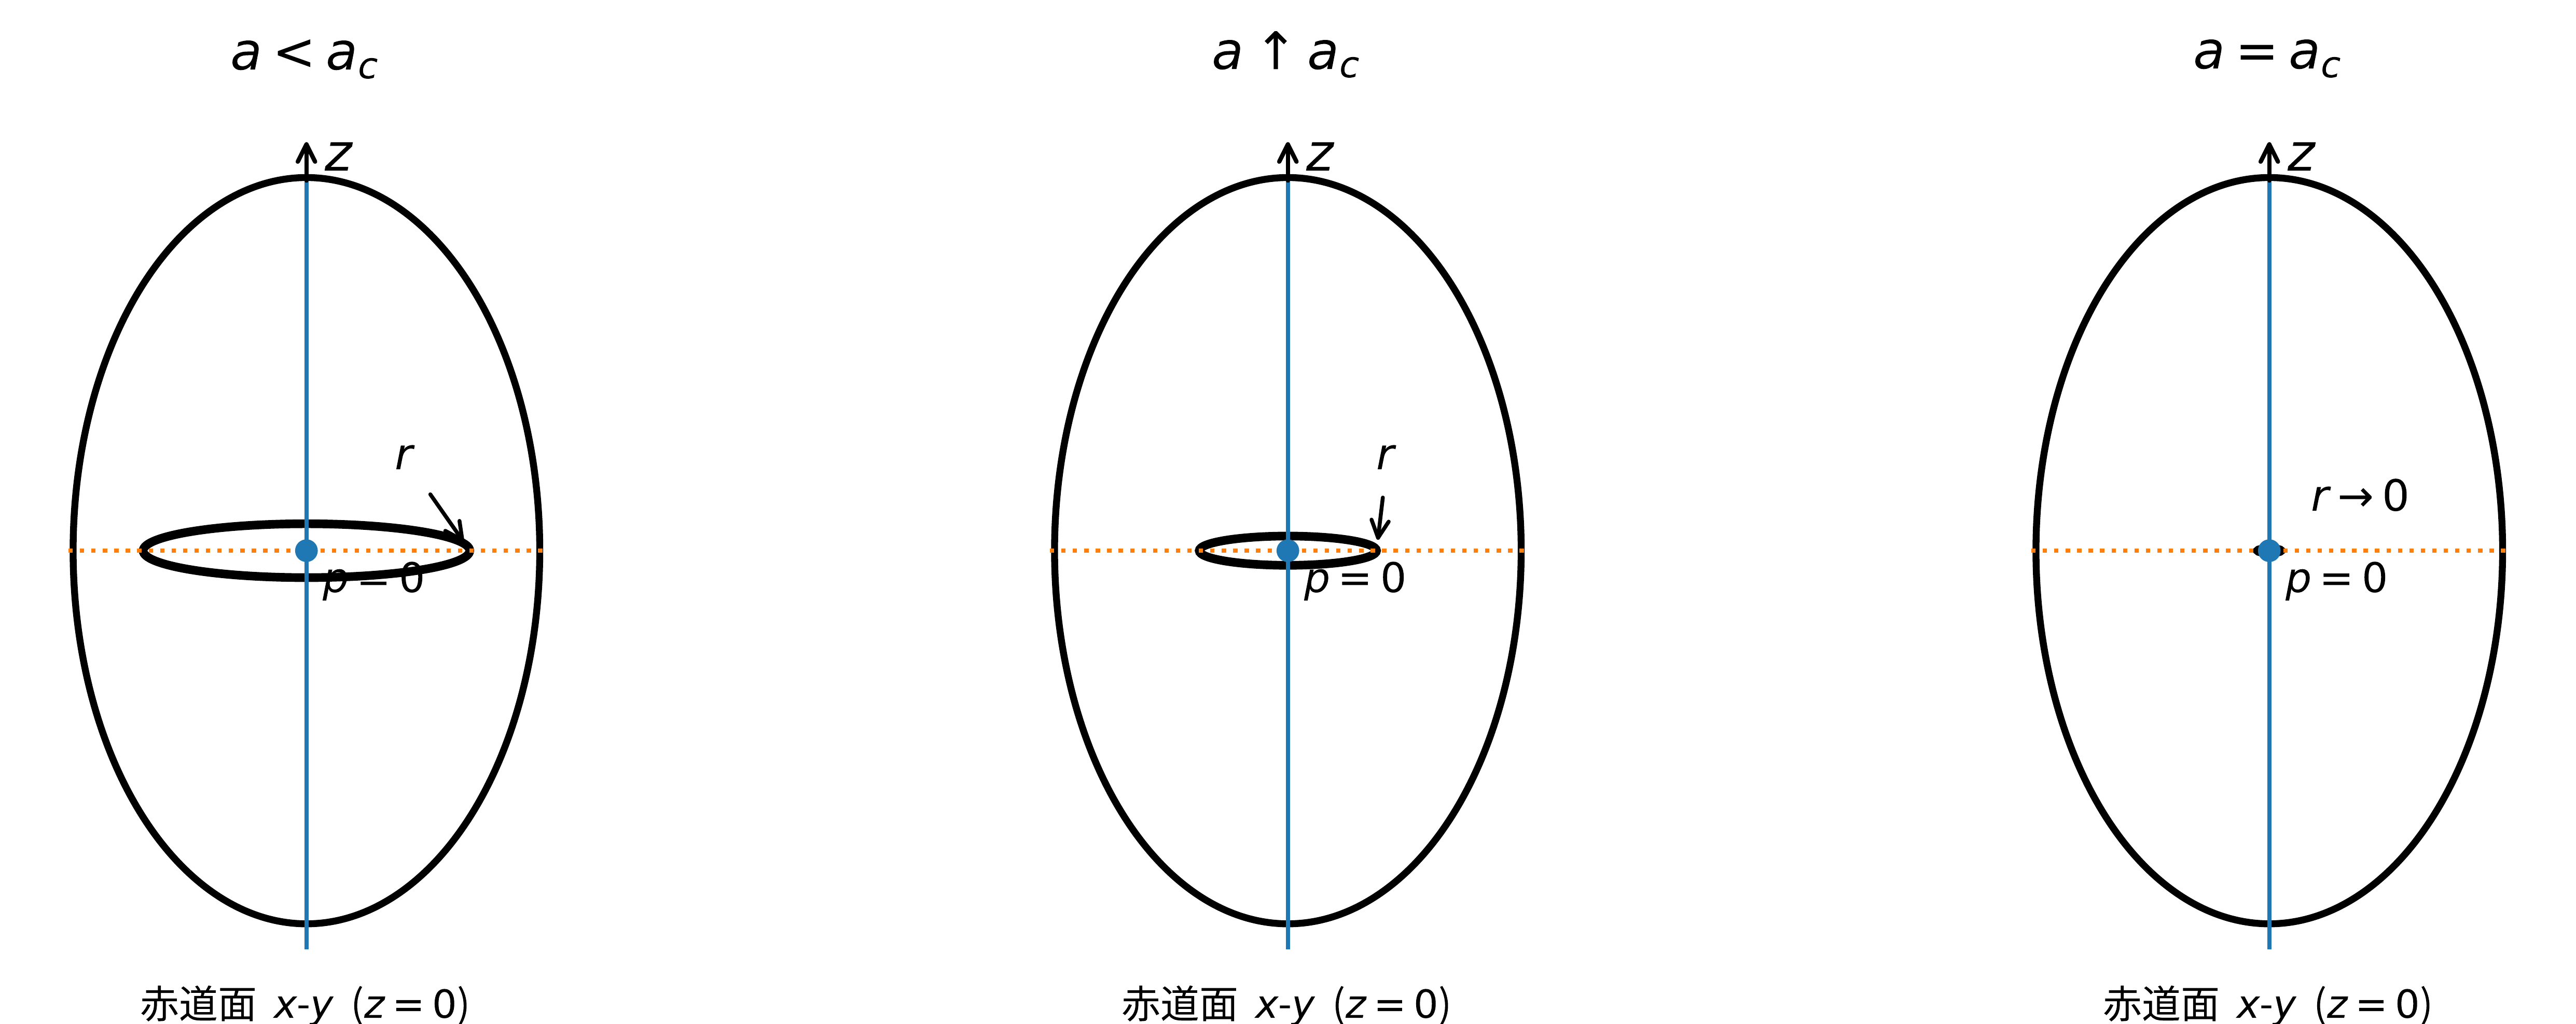
\includegraphics[width=\linewidth]{figures/fig2_shrinking_circle.png}
\caption{停留円の中心への収縮を示す幾何学的模式図。回転軸は \(z\) 軸、赤道面は \(x\)–\(y\) 平面
（\(z=0\)）である。停留円は赤道面内にあり、\(a\uparrow a_c\) に伴って軌道半径 \(r\) は零へ近づき、
臨界値で中心に合流する。形状・半径・軸比は説明のための模式表現であり、縮尺には従わない。}
\label{fig:shrink}
\end{figure}

\(a_c\) を内点に含む十分小さい両側区間 \(I\) を取る。\(a<a_c\) に属する \(I\) の片側では、赤道面に
半径 \(r(a)>0\) の一意な停留円 \(C_a\) が存在する。円は \(D_{\infty h}\) の軸方向 \(O(2)\) 部分群に
よる一つの軌道であり、その各点の等方群は全群で固定される中心の等方群と異なる。接方向の零モードは
群作用に由来し、法方向 Hessian が非退化であれば \(C_a\) は Morse–Bott 臨界多様体となる。

臨界値の反対側では、中心の同じ局所近傍に非零停留円は存在せず、中心成分のみが残る。したがって局所
停留集合の芽は、一側で「孤立中心＋一次元円成分」、他側で「孤立中心」へ変わる。成分次元の変化だけで
ラベル保存局所自明性は破れる。さらに \(a=a_c\) では \(Q(a_c)=0\) により中心 Hessian の赤道方向
固有空間が核に入り、中心成分の nullity も変化する。これは成分次元の変化とは独立な第二の分岐証拠で
ある。

\leadin{重要な限定。}
ここで証明するのは \((a_c,0)\) における局所的な基点分岐の存在である。軸比全域のすべての停留成分を
列挙したとは主張しない。完全な三次元ラベル表の認証は主定理の前提ではなく、続編の課題である。

\section{主定理：基点分岐の存在}
\begin{thm}[扁長回転楕円体における局所基点分岐]
\label{thm:main}
錐体積重み付き動径–法線角汎関数 \(E_a\) に対し、\((a_c,0)\in\mathcal{S}\) は基点分岐点であり、
\(a_c\in(4.72438,4.72439)\) は基点分岐値である。すなわち、\(a_c\) を内点に含む任意に小さい両側近傍
\(I\) と中心 \(0\) の任意に小さい近傍 \(U\) に制限した射影
\(\pi:\mathcal{S}\cap(I\times U)\to I\) は、ラベル保存局所自明ではない。具体的には、解析的陰関数定理で得られる
赤道面内の局所停留枝について、\(a_c\) の一側に一次元の停留円成分が存在して中心へ収縮するのに対し、
他側の対応する局所近傍にはその成分が存在しない。さらに \(a_c\) では中心 Hessian の nullity が増加する。
\end{thm}

\section{計算機援用認証の役割}
本稿の主定理に必要な計算機援用部分は、\(Q\) の零点区間、\(Q'\) の符号および \(H_4\) の符号を認証する
局所係数計算である。探索段階で候補区間を得た後、閉区間上の外向き丸めにより各符号を固定し、解析的な
局所分岐議論へ接続する。

\section{既存中心理論との関係}
中心の理論は点を見てきた。本研究は軌道を認証する。

\section{射程と続編との境界}
本稿の責任範囲は存在である。すなわち、\((a_c,0)\) の芽に少なくとも一つの基点分岐があり、その任意に
小さい近傍でラベル構造が変わることを示す。軸比の全域を被覆し、すべての停留成分とすべての分岐値を
完全列挙することは要求しない。

\section{展望}
三軸楕円体へ対称性を破ると、扁長回転楕円体の停留円は四つの孤立停留点へ分裂し、完全な点群は
\[
D_{\infty h}\longrightarrow D_{2h}
\]
へ移ると予想される。

\section{結論}
扁長回転楕円体に付随する錐体積重み付き動径–法線角について、中心近傍の停留構造を解析し、臨界軸比の
一側に停留円が存在して中心へ収縮することを認証した。

\section*{Acknowledgments}
著者は、Jonathan Borwein と David Bailey が示した実験数学の理念から受けた影響に深い敬意を表する
\cite{BorweinBailey}。

\appendix

\section{計算機援用証明の再現情報}
\begin{itemize}
\item 正典数式の記号監査：\path{CERTIFICATES/prolate/local_bifurcation/prolate_B2_symbolic_audit.py}
      および \path{prolate_H4_symbolic_audit.py}。各 SHA-256 は同ディレクトリの
      \path{SHA256SUMS.txt} に固定する。
\item 区間演算、丸め、入力区間および実行設定：
      \path{CERTIFICATES/prolate/local_bifurcation/prolate_cap_arb_certificate.py}。
\item 包含証明出力：
      \path{CERTIFICATES/prolate/local_bifurcation/prolate_cap_arb_certificate.json}
      （\texttt{status=CERTIFIED}、6条件すべて true）。
\item 座標規約。認証スクリプトで用いる球面角 \(\theta\) は、本文 §4 の回転軸である \(z\) 軸を基準と
      する極角である。したがって \(\ell=\sin^2\theta+a^2\cos^2\theta\) における \(\cos\theta\) は
      伸長軸方向に対応し、\(u=\sin\theta\cos\phi\) は赤道面内の横断方向成分に対応する。
\item 再現スクリプト、証明出力および SHA manifest の archival commit（リポジトリ \cite{Repo}）：\\
      \texttt{9d23185e571deea67fe7c3a33573b62cf61593e7}
\end{itemize}

\section{局所係数 \(Q\) および \(H_4\) の正典表示}
\label{app:canonical-kernels}
本付録では、本文で用いた局所係数 \(Q(a)\) と \(H_4(a)\) を、認証コードと同一の一変数核として明示する。
扁長回転楕円体 \(K_a\) に対し、赤道方向の基点を
\[
p_r=(r,0,0)
\]
と置く。球面角は本文と同じく \(z\) 軸を極軸とし、
\[
s=\sin\theta,\qquad c=\cos\theta,\qquad
u=s\cos\phi,
\]
\[
\ell=s^2+a^2c^2,\qquad
W=\sqrt{a^2s^2+c^2},\qquad
C=\frac{a}{W\sqrt{\ell}}
\]
とする。さらに
\[
h(x)=\arccos(x)^2
\]
と置くと、正規化後の角度部分に現れる余弦は
\[
\gamma(r)=C(1-ru)
\left(1-\frac{2ru}{\ell}+\frac{r^2}{\ell}\right)^{-1/2},
\]
重みを含む \(r\)-依存核は
\[
F(r)=(1-ru)h(\gamma(r))
\]
である。

\subsection{端点正則化と積分記号下の微分}
\begin{prop}[端点を含む微分の正当化]
\label{prop:diff-under-integral}
\(a\) を \([4.7,4.75]\) の閉部分区間に制限する。このとき上記核は \(r=0\) の近傍で \(r\) に関して
4階まで微分可能であり、その各導関数は \(\theta\in[0,\pi/2]\) 上で連続な可積分関数として延長される。
したがって \(r\) に関する2階および4階微分を積分記号の下へ移すことができる。
\end{prop}

\begin{proof}
認証実装では \(\beta=\arctan t\), \(t=(a-a^{-1})sc\), \(z=\beta^2\) と置き、
\[
S={}_0F_1\!\left(;\frac32;-\frac z4\right),\quad
T={}_0F_1\!\left(;\frac52;-\frac z4\right),\quad
U={}_0F_1\!\left(;\frac72;-\frac z4\right),\quad
V={}_0F_1\!\left(;\frac92;-\frac z4\right)
\]
を用いる。\(h_j=h^{(j)}(C)\) は cancellation-free な形
\begin{align*}
h_1&=-\frac{2}{S},\\
h_2&=\frac{2}{3}\frac{T}{S^3},\\
h_3&=\frac{2}{15}\frac{U}{S^4}-\frac{2}{3}\frac{T^2}{S^5},\\
h_4&=\frac{2}{105}\frac{V}{S^5}-\frac{4}{9}\frac{UT}{S^6}
      +\frac{10}{9}\frac{T^3}{S^7}
\end{align*}
で評価される。これらは \(\beta=0\) でも正則であり、端点カットオフや別個の Taylor chart を必要としない。
また \(a\in[4.7,4.75]\) では \(\ell>0\) と \(W>0\) が一様に成り立つ。したがって必要な導関数は
コンパクト集合上で連続かつ一様有界であり、通常の優収束による積分記号下微分が適用できる。
\end{proof}

\subsection{二次係数 \(Q\)}
\(h_1=h'(C)\), \(h_2=h''(C)\) と書く。\(F\) を \(r\) で2回微分し \(r=0\) とすると、点ごとに
\[
F''(0)=\frac{C}{\ell^2}\left[
C h_2(\ell-1)^2u^2
+h_1\bigl((2\ell^2-4\ell+3)u^2-\ell\bigr)
\right].
\]
ここで
\[
\int_0^{2\pi}1\,d\phi=2\pi,\qquad
\int_0^{2\pi}u^2\,d\phi=\pi s^2
\]
を用いると、正典の一変数核
\[
B_2(\theta,a)=\frac{C}{\ell^2}\left[
C h_2(\ell-1)^2s^2
+h_1\bigl((2\ell^2-4\ell+3)s^2-2\ell\bigr)
\right]
\]
を得る。したがって
\[
\boxed{Q(a)=\frac12\int_0^{\pi/2}s\,B_2(\theta,a)\,d\theta .}
\]

\subsection{四次係数 \(H_4\)}
\(h_j=h^{(j)}(C)\)（\(j=1,\dots,4\)）とする。4階微分は
\[
F^{(4)}(0)=A_4u^4+A_2u^2+A_0
\]
と厳密に分解され、奇数次の \(u\) 項は恒等的に消える。各係数は
\begin{align*}
A_4={}&\frac{C}{\ell^4}\Bigl[
C^3h_4(\ell-1)^4
+C^2h_3(4\ell^4-24\ell^3+54\ell^2-52\ell+18)\\
&\qquad +Ch_2(-24\ell^3+108\ell^2-168\ell+87)
+h_1(36\ell^2-120\ell+105)\Bigr],\\
A_2={}&-\frac{6C}{\ell^3}\Bigl[
C^2h_3(\ell-1)^2+Ch_2(4\ell^2-12\ell+9)
+h_1(2\ell^2-12\ell+15)\Bigr],\\
A_0={}&\frac{3C}{\ell^2}(Ch_2+3h_1).
\end{align*}
さらに
\[
\int_0^{2\pi}u^4\,d\phi=\frac{3\pi}{4}s^4,\qquad
\int_0^{2\pi}u^2\,d\phi=\pi s^2
\]
より、正典の一変数核は
\[
B_4(\theta,a)=\frac34A_4s^4+A_2s^2+2A_0
\]
となる。したがって
\[
\boxed{H_4(a)=\frac12\int_0^{\pi/2}s\,B_4(\theta,a)\,d\theta .}
\]

\subsection{認証包絡値}
表1は、\path{prolate_cap_arb_certificate.json} に保存された Arb/Acb ball の実部包含を、読みやすさのため
外向きに丸めて再掲したものである。計算精度は50桁、積分 tolerance は \(10^{-20}\)、パラメータ区間
\([4.7,4.75]\) は5分割である。

\begin{table}[htbp]
\centering
\small
\caption{局所係数の認証包絡。表示値は JSON の厳密 ball 包含を外向きに丸めたもの。}
\begin{tabular}{lll}
\hline
対象 & \(a\) または区間 & 認証包含 \\
\hline
\(Q\) & \(4.72438\) & \([3.22198042890824\times10^{-7},\,3.22198042890832\times10^{-7}]\) \\
\(Q\) & \(4.72439\) & \([-6.24183175809915\times10^{-7},\,-6.24183175809908\times10^{-7}]\) \\
\hline
\(Q'\) & \([4.70,4.71]\) & \([-0.10545,-0.08573]\) \\
\(Q'\) & \([4.71,4.72]\) & \([-0.10492,-0.08527]\) \\
\(Q'\) & \([4.72,4.73]\) & \([-0.10438,-0.08480]\) \\
\(Q'\) & \([4.73,4.74]\) & \([-0.10386,-0.08434]\) \\
\(Q'\) & \([4.74,4.75]\) & \([-0.10333,-0.08388]\) \\
\hline
\(H_4\) & \([4.70,4.71]\) & \([-1.49670,-1.39252]\) \\
\(H_4\) & \([4.71,4.72]\) & \([-1.49333,-1.38959]\) \\
\(H_4\) & \([4.72,4.73]\) & \([-1.48998,-1.38666]\) \\
\(H_4\) & \([4.73,4.74]\) & \([-1.48664,-1.38375]\) \\
\(H_4\) & \([4.74,4.75]\) & \([-1.48331,-1.38085]\) \\
\hline
\end{tabular}
\end{table}

\begin{thebibliography}{99}
\small
\bibitem{BorweinBailey}
J.~M. Borwein and D.~H. Bailey,
\textit{Mathematics by Experiment: Plausible Reasoning in the 21st Century},
A~K Peters, Natick, MA, 2004.

\bibitem{GSS}
M.~Golubitsky, I.~Stewart, and D.~G. Schaeffer,
\textit{Singularities and Groups in Bifurcation Theory}, Vol.~II,
Applied Mathematical Sciences 69, Springer, New York, 1988.

\bibitem{Repo}
K.~Furuta,
``Basepoint Geometry: computational certificates for the prolate-spheroid basepoint bifurcation,''
software and proof archive, GitHub,
archival commit, 2026.\\
\texttt{9d23185e571deea67fe7c3a33573b62cf61593e7}.
Repository URL: \url{https://github.com/cotaxxxx/basepoint-geometry}.
Version DOI (Zenodo): \textbf{[PENDING — Zenodo version DOI 取得後に記入]}.
\end{thebibliography}

\end{document}